\documentclass{standalone}
%\usepackage{scrtime} % for \thistime (this package MUST be listed first!)
\usepackage{graphicx}
\usepackage{graphics}
\usepackage{xcolor,colortbl}%for changing cell colour
\usepackage{xspace}
\usepackage{tikz-cd}
\usetikzlibrary{decorations.markings}
\usetikzlibrary{calc, arrows}
\usepackage{color,amsmath,amssymb,amsthm,mathrsfs,amsfonts,dsfont}


\begin{document}
	\centering{
	\resizebox{\textwidth}{!}{%
		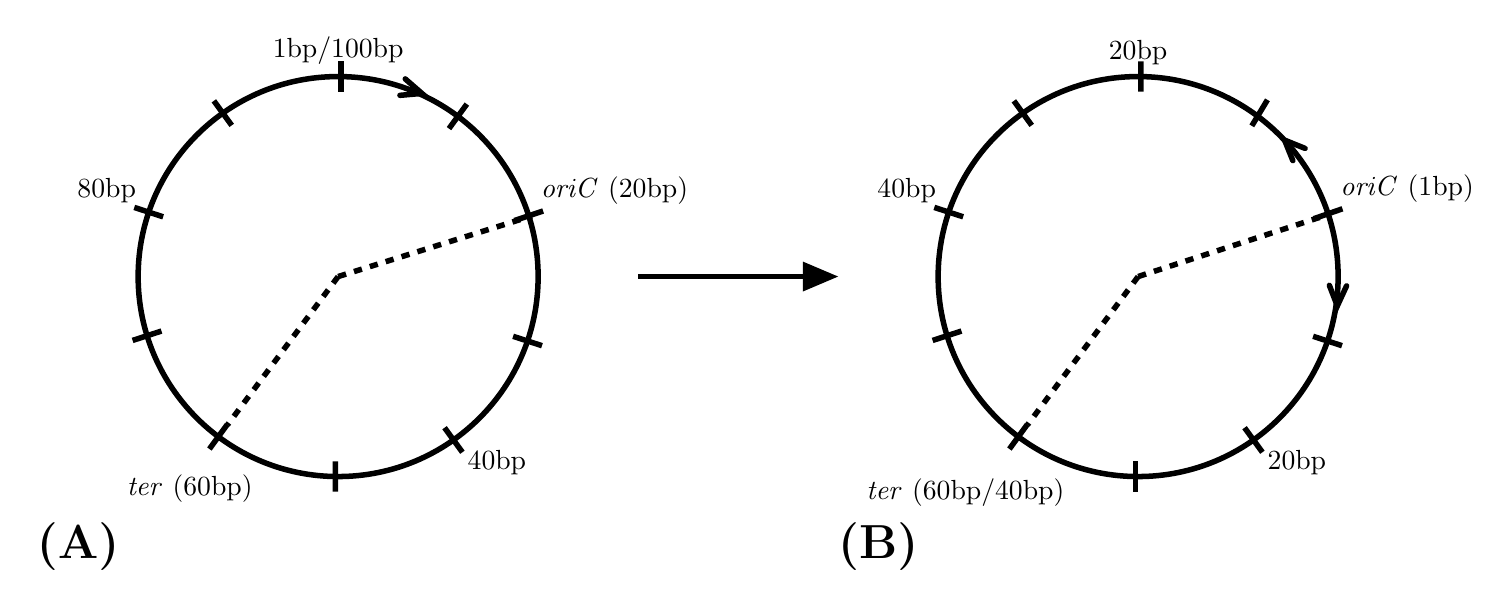
\begin{tikzpicture}[x=1in, y=1in]
		%circle on left
		\draw[line width=0.7mm,
		decoration={markings, 	
			%the position below denotes the distance from the right most point of the circle (3 on a clock) going counter clock wise 1= 3oclock position
			%arrow for "replication" direction
			mark=at position 0.2 with {\arrow[>=angle 45]{<}},
			%oriC tick
			mark=at position 0.0513 with {\arrow[line width=0.7mm]{|}},
			%oriC node
			mark=at position 0.049 with \node[above right](ori){\textit{oriC} (20bp)};,
			%10bp tick
			mark=at position 0.15 with {\arrow[line width=0.7mm]{|}},
			%position 90 tick
			mark=at position 0.35 with {\arrow[line width=0.7mm]{|}},
			%position 0/100 tick
			mark=at position 0.25 with {\arrow[line width=0.7mm]{|}},
			%position 0/100 node
			mark=at position 0.25 with \node[above](pos0){1bp/100bp};,
			%80bp tick
			mark=at position 0.45 with {\arrow[line width=0.7mm]{|}},			
			%80bp node
			mark=at position 0.45 with \node[above left](pos80){80bp};,
			%70bp tick
			mark=at position 0.55 with {\arrow[line width=0.7mm]{|}},
			%ter tick
			mark=at position 0.65 with {\arrow[line width=0.7mm]{|}},		
			%ter node lab
			mark=at position 0.648 with \node[](ter){};,
			%ter node lab
			mark=at position 0.69 with \node[below left]{\textit{ter} (60bp)};,
			%30bp tick
			mark=at position 0.95 with {\arrow[line width=0.7mm]{|}},
			%40bp tick
			mark=at position 0.85 with {\arrow[line width=0.7mm]{|}},
			%40bp node
			mark=at position 0.85 with \node[below right](pos40){40bp};,
			%50bp tick
			mark=at position 0.75 with {\arrow[line width=0.7mm]{|}},
		},
		postaction={decorate}] (1.5,1.5) circle (1in);
		%arrow between circles
		\draw[->,line width=0.7mm, >=triangle 45] (3,1.5) -- (4,1.5);
		%line btwn origin and middle of circle
		\draw[line width=0.7mm, dashed] (1.5,1.5) -- (ori);
		%line btwn ter and middle of circle
		\draw[line width=0.7mm, dashed] (1.5,1.5) -- (ter);
		%circle to the right
		\draw[line width=0.7mm,
		decoration={markings, 	
			%the position below denotes the distance from the right most point of the circle (3 on a clock) going counter clock wise 1= 3position
			%arrow for "replication" direction #1
			mark=at position 0.125 with {\arrow[>=angle 45]{>}},
			%oriC tick
			mark=at position 0.053 with {\arrow[line width=0.7mm]{|}},
			%oriC node
			mark=at position 0.05 with \node[above right](ori2){\textit{oriC} (1bp)};,
			%position 90 tick
			mark=at position 0.35 with {\arrow[line width=0.7mm]{|}},
			%40 tick
			mark=at position 0.45 with {\arrow[line width=0.7mm]{|}},
			%position 40 node
			mark=at position 0.45 with \node[above left](2pos80){40bp};,
			%position 0/100 tick
			mark=at position 0.25 with {\arrow[line width=0.7mm]{|}},
			%position 0/100 node
			mark=at position 0.25 with \node[above](2pos0){20bp};,
			%10 tick
			mark=at position 0.15 with {\arrow[line width=0.7mm]{|}},	
			%ter node lab
			mark=at position 0.70 with \node[below left](ter2){\textit{ter} (60bp/40bp)};,
			%ter node
			mark=at position 0.648 with \node[](terr){};,
			%50 tick
			mark=at position 0.55 with {\arrow[line width=0.7mm]{|}},
			%ter tick
			mark=at position 0.65 with {\arrow[line width=0.7mm]{|}},
			%position 40 tick
			mark=at position 0.85 with {\arrow[line width=0.7mm]{|}},
			%30 tick
			mark=at position 0.95 with {\arrow[line width=0.7mm]{|}},
			%50 tick
			mark=at position 0.75 with {\arrow[line width=0.7mm]{|}},
			%40 node
			mark=at position 0.85 with \node[below right](2pos40){20bp};,
			%arrow for "replication" direction #2
			mark=at position 0.995 with {\arrow[>=angle 45]{<}}
		},
		postaction={decorate}] (5.5,1.5) circle (1in);
		%line btwn origin and middle of circle
		\draw[line width=0.7mm, dashed] (5.5,1.5) -- (ori2);
		%line btwn ter and middle of circle
		\draw[line width=0.7mm, dashed] (5.5,1.5) -- (terr);
		%fig lable A
		\node[] at (0.2,0.15) {\LARGE \textbf{(A)}};
		%fig lable B
		\node[] at (4.2,0.15) {\LARGE \textbf{(B)}};
		\end{tikzpicture}
	}%resiebox
}

	\end{document}